%---------------------------------------------------------------------------
% Chapter 2 - Similar techonologies
%
%---------------------------------------------------------------------------
 
 
\section{Overiew of simillar monitoring systems}
\label{sec:ch2_similar}


%---------------------------------------------------------------------------
\subsection{perfSonar}

perfSonar (\cite{perfSonar1,perfSonar2,perfSonar3}) is an infrastructure for network performance monitoring. It aims in making process of
solving end-to-end performance problems on paths that crosses several networks easier. It is composed of a set of services delivering
performance measurements in federated environment. This approach allows to classify project as a middlewere service, that is in use by
performance measuring tools and diagnostic or visualization applications. The layer created by perfSonar aims to make and exchange of 
measurement data between networks, using well defined protocols.  Architecture of perfSONAR is service oriented, which means that the
set of elementary functions (\emph{services}) has been isolated and can be provided by several, independent entities.

Work done on perSONAR is made around three contexts. First, there is a consortium of organizations that build network of performance
middleware that is interoperable across multiple networks and useful for variate network analysis. The second context is a protocol. It is build on
assumption of fixed, well defined roles (service types) and defines communication between components implementing each role. Such a approach
allows interoperability. What is also worth mentioning, protocol is based on SOAP XML messages format and follows Network
Measurement Working Group\footnote{\url{http://nmwg.internet2.edu}} schema.  The third context is set of implemented software packages that
provide those services.

The framework defines following types of services:

\begin{itemize}
\item{ {\bf Measurement Point Service}, acts as a service provider. Standard doesn\rq{}t define whether it gathers measurement values
dynamically, by querying measured components or retrieves static, archived data. It defines only role of this component as a source of
measurement values.}
\item{ {\bf Measurement Archive Service}, is responsible for archivization. It can use any storage facility underneath (Round Robin Database or
any RDBMS). Additionally it can publish received information. }
\item{ {\bf Lookup Service}, enables services to discover each other. It acts as service directory, where providers can advertise themselves and
requestors are able to find any service needed}
\item{ {\bf Authentication Service}, helps domains which would like to restrict access to given service capabilities for some groups of users. It is
responsible for both authorization (who is given user) and authentication - it acts as, so called, attribute authority (decides which attribute can be 
disclosed to a resource)}
\item{ {\bf Transformation Service}, is generic service type that allows creation of data conversion pipelines. It is able to perform any function
upon data taken from producer and returns transformed data to consumer}
\item{ {\bf Topology Service}, provides the framework informations about network topology, which allows for example visualization of network
maps. Additionally it gives information on geolocation, like GPS coordinates.}
\item{ {\bf Resource Protector Service} - it is used to arbitrate the consumption of limited, shared resources (like network bandwidth).}
\end{itemize}

%---------------------------------------------------------------------------
\subsection{SCALEA and SCALEA-G}

SCALEA~\cite{SCALEA1} is a tool for instrumentation, measurement, analysis and visualization of execution of parallel programs. It can work with
OpenMP, MPI, HPF, and mixed parallel/distributed programs. It measurements are based on a variety of performance metrics, but SCALEA
also supports multiple experiment performance analysis that allows to compare and to evaluate the performance
outcome of several experiments.

Architecture of system distinguishes three main components: SCALEA Instrumentation System (\emph{SIS}),
SCALEA Runtime System (\emph{SRS}) and SCALEA
Performance Analysis \& Visualization System. SIS can instrument any of: Fortran, OpenMP, MPI, HPF or even
hybrid programs like OpenMP/MPI and allows user to select code regions and performance metrics of interest. Using this input, SIS inserts probes
in the code which will collect all relevant performance information. Those data are saved in a set of profile (trace) files during program execution,
which is monitored by SRS. Additionally, SIS generates,  instrumentation description file, that can be used to associate gathered performance data
back to the input program. Performance Analysis \& Visualization sub system can use gathered raw data either during the program execution, or
post-mortem.

The main purpose of SCALEA-G (\cite{SCALEA2, SCALEA3}) is to bring functionality of SCALEA to the grid
environment. Originally it was implemented as a set of OGSA services based on Globus Toolkit 3.0, but it was
ported then into WSRF-based services with Globus Toolkit 4.0. The most recent implementation of SCALEA-G is
composed of following services:

\begin{itemize}
\item{ {\bf Registry Service}}
\item{ {\bf Directory Service}}
\item{ {\bf Sensor Manager Service} - monitors and measures performance of Grid services. Internally, it is
implemented as WSRF-based service that collects monitoring data from sensors. It supports 2 communication
modes - either query/request and subscribe/notify. Collected data are stored in XML containers, based on DBXML.
The sensors can be monitor system, application or used other tools, like NWS, Iperf or Ganglia.}
\item{ {\bf Dynamic Instrumentation Service}, used for instrumentation of native application. It uses internally C++ gSOAP+, GSI-plugin and Dyninst}
\item{ {\bf XML data schema Service}}
\item{ {\bf Client Service}}
\item{ {\bf GUI Component}}
\item{ {\bf Set of Java APIs}}
\end{itemize}


%---------------------------------------------------------------------------
\subsection{DIPAS}

DIPAS~\cite{DIPAS}, which stands for DIstributed Performance Analysis Service, is an monitoring platform
designed to work with K-WfGrid (see section~\ref{ssec:kwfgrid}). The aim of this project is to provide on-line
information about the performance of Grid workflows as well as Grid resources involved in the it\rq{}s execution. Those informations are used not only by user, but it also gives to the K-WfGrid middleware and services
source of knowledge about the performance, which improves the process of semi-automatic workflow
construction.

DIPAS provides performance analysis and interpretation for workflows which is based on a novel classification of
performance overheads. It allows user to define the performance constraints and using this input DIPAS informs the user and client about potential performance problems by interpreting metrics at runtime.
Performance analysis of workflows is integrated with tools built-in to the Grid infrastructure, creating coherent
framework. 

Additionally, DIPAS provides a Web portal for the user to conduct performance monitoring and analysis of workflows and infrastructure, thus substantially simplifying the way the user interacts with the tool.

Overall architecture of system is outlined in Figure~\ref{fig:dipas}

\begin{figure}[ht]
  \centering
  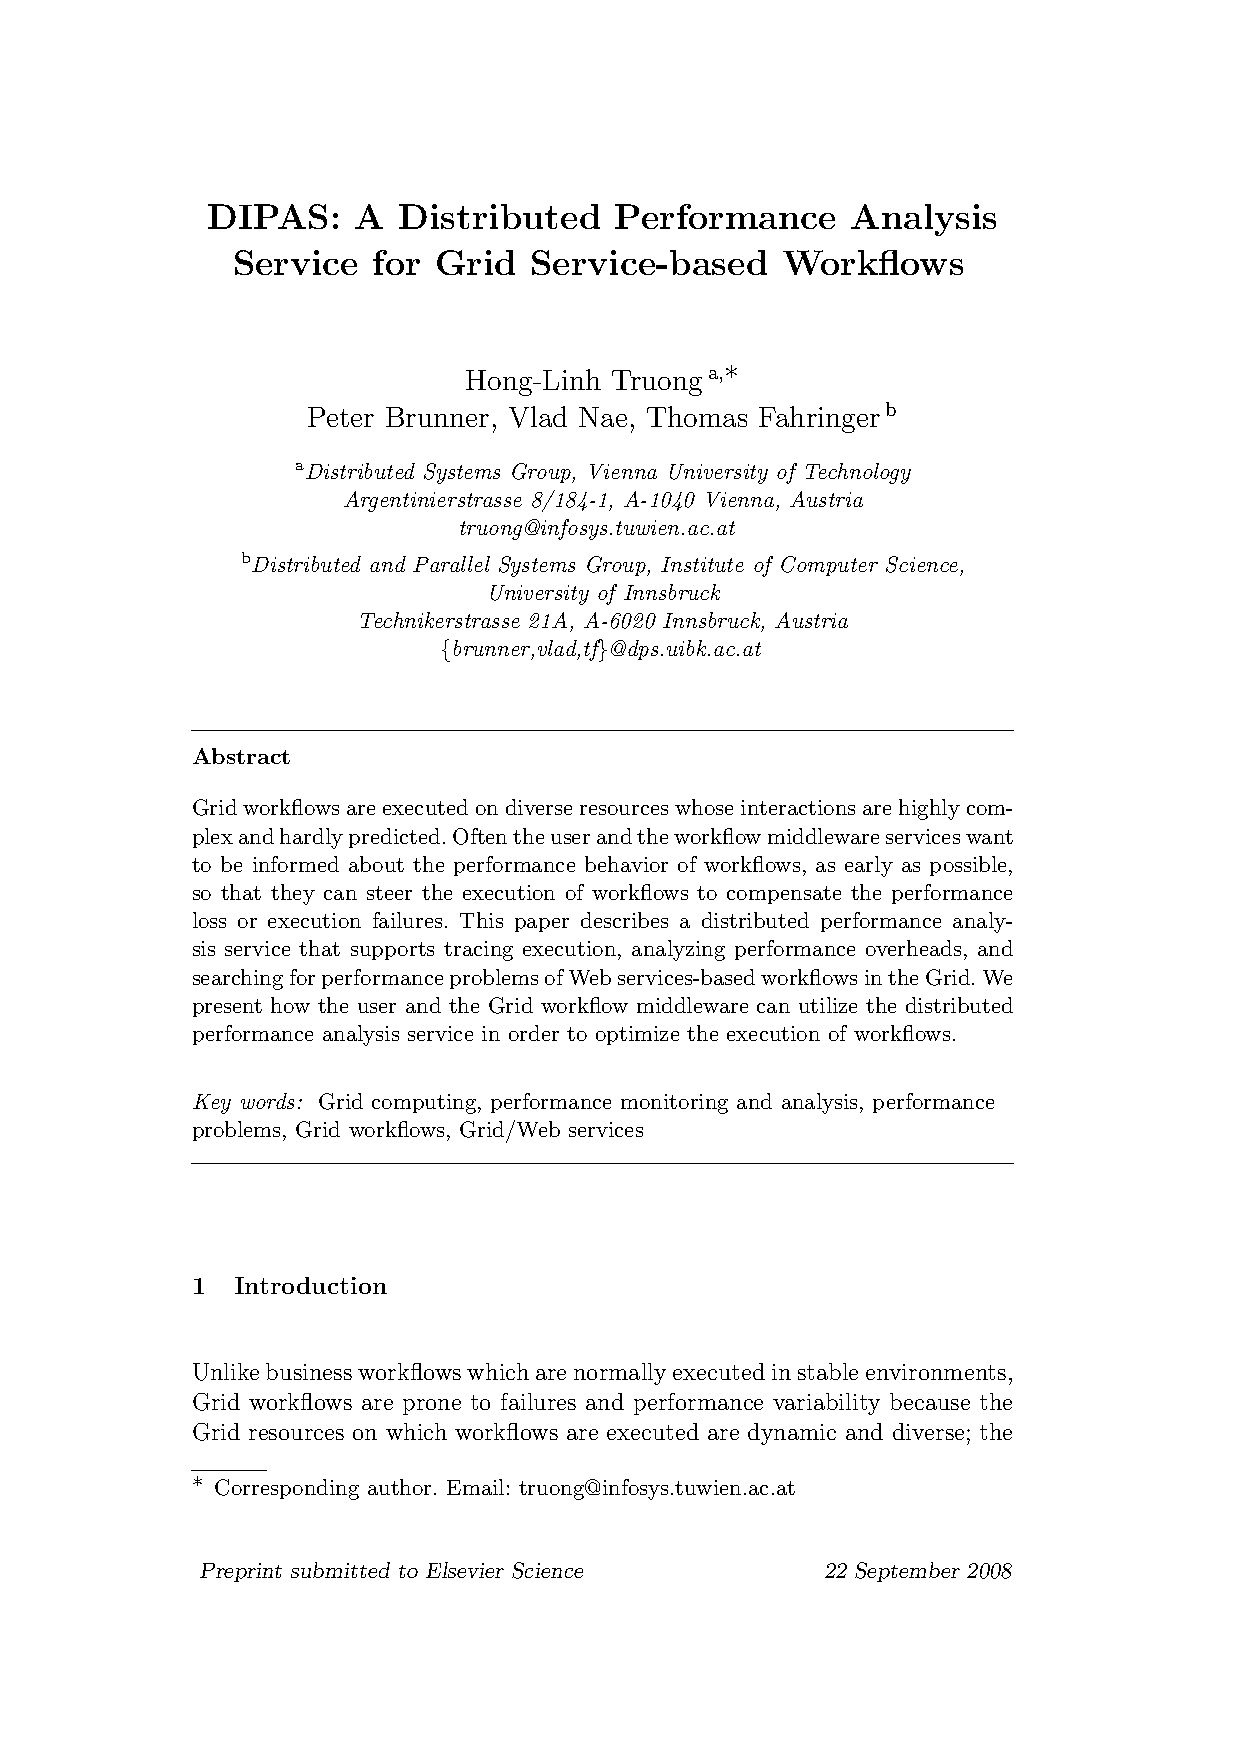
\includegraphics[width=0.6\textwidth]{dipas}
  \caption{Overall architecture of DIPAS}
  \label{fig:dipas}
\end{figure}

%---------------------------------------------------------------------------
\subsection{OCM Family}

As part of work on OMIS (See section~\ref{ssec:omis}) several tools that are compliant with this interface where introduced. This tool set
includes: OCM\footnote{\url{http://www.lrr.in.tum.de/Par/tools/Projects/OCM.html}}, OCM-G\footnote{\url{http://grid.cyfronet.pl/ocmg}}, J
OCM\footnote{\url{http://jocm.icsr.agh.edu.pl/sub/main}} and G-PM\footnote{\url{http://gpm.icsr.agh.edu.pl}}.

OCM (\cite{RWspdt98, RW:ppam99b}) - OMIS Compliant Monitoring System is the first tool in whole set. The main goal of this project was to create a reference implementation of an OMIS compliant monitoring system. Initially it supported PVM (versions 3.3 and 3.4) and MPI-1. 

As a next step in platform evolution, OCM-G, which states for Grid-enabled OMIS-Compliant Monitoring system (\cite{axgrid03b}) was introduced.
This project focuses on using OMIS interface with grid environments.  In spite of working with well known MPI parallel programming library, it was
designed to work with Globus Toolkit and is fully compliant with EGEE environment including gLite 3.x\footnote{\url{http://glite.cern.ch/}} and LCG
2.7. 

The last addition to set OMIS-compliant tools is J-OCMG - Java oriented monitoring infrastructure (\cite{jocm}). It adds ability of monitoring JVM
based applications. It extended standard OMIS interface with a set of new, Java-specific services, like garbage collection, threads execution, class
loading or method invocation. Currently project implementation focuses on monitoring Java Web Services and component oriented applications.

General architecture shared among all mentioned above systems can be found in Figure~\ref{fig:ocmg}.

\begin{figure}[ht]
  \centering
  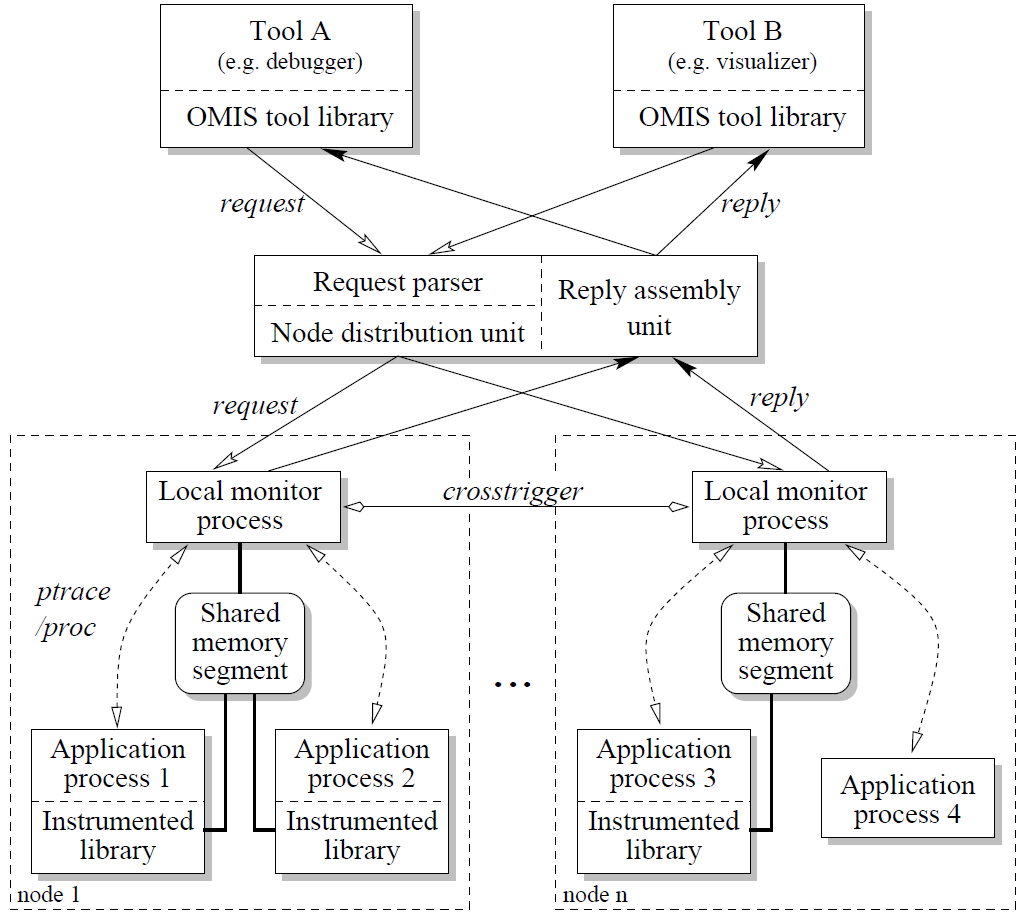
\includegraphics[width=0.8\textwidth]{ocm_arch}
  \caption{Common OMIS-compliant tools architecture diagram}
  \label{fig:ocmg}
\end{figure}
 
%---------------------------------------------------------------------------
\subsection{R-GMA}

R-GMA: Relational Grid Monitoring Architecture~(\cite{RGMA1,RGMA2,RGMA3}) is implementation of GMA, described in section~\ref{ssec:gma}.
Although it implements GMA interface, it adds two exceptions to the standard. First, anyone supplying or obtaining information from R-GMA does
not need to know about the Registry component, as it\rq{}s responsibility is processed by Consumer and Producer components \lq\lq{}behind the
scenes\rq\rq{}. The second exception is that information and monitoring system appears to the end user, like one large relational database and can be queried as such. It is the source of R (Relational) in project name.

All systems using R-GMA share information in a virtual database, with data organized into tables, and managed using standard SQL constructs (like
INSERT INTO... or SELECT FROM). Regarding internal database structure, there is no central repository that actually holds the data for each
table. Virtual database just consists of a list of table definitions (\emph{schema}), a list of data providers (\emph{registry}) and a set of rules for
deciding which data providers needs to be used while preparing result for given query. These rules are fixed and encoded into a internal
component called \emph{mediator}.

The system provides several ways to access the database. There are provided API, with bindings available in Java, C/C++ and Python. Additionally
users can work with database using web interface or command line utility.
